\documentclass{article}
\usepackage[ruled, linesnumbered]{algorithm2e}
\def\showtopic{Numerical Analysis}
\def\showtitle{Lab 5: Numerical ODE}
\def\showabs{Lab 5}
\def\showauthor{Ting Lin, 1700010644}
\def\showchead{LIN}
\usepackage{amsmath, amsfonts, amsthm}

\usepackage{graphicx, epstopdf}
\usepackage{color}
\usepackage{geometry, graphicx}
\usepackage{algorithm, algorithmic}
\usepackage{bm}
\usepackage{multirow}
\usepackage{ulem}
\geometry{left = 5em, right = 5em}
\usepackage{listings}
\usepackage{xcolor}
%% notation macro
\newcommand{\F}{\mathcal F}
\newcommand{\T}{\mathcal T}
\newcommand{\I}{\mathcal I}
\newcommand{\U}{\mathcal U}
\newcommand{\R}{\mathbb R}
\renewcommand{\P}{\mathcal P}
\newcommand{\uP}{ \mathcal \uline P}
\newcommand{\B}{\mathcal B}
%\newcommand{\R}{\mathbb R^2}
\newcommand{\Z}{\mathbb Z}
\newcommand{\C}{\mathbb C}
\newcommand{\laplacian}{\triangle}
\newcommand{\grad}{\nabla}
\renewcommand{\div}{\textrm{div~}}

\newcommand{\diff}[2]{\frac{\partial #1}{\partial #2}}
\newcommand{\difff}[3]{\frac{\parial #1^2}{\partial #2 \partial #3}}
\newcommand{\diFF}[2]{\frac{\partial #1^2}{\partial^2 #2}}
\newcommand{\diam}{\text{ diam }}
%% non-noation macro
\newcommand{\IN}{\text{  in  }}
\newcommand{\ON}{\text{  on  }}
\newcommand{\st}{\text{s.t.  }}
\newcommand{\tbc}{{\color{red}[TBC]}}

%% enviorment
\newtheorem{proposition}{Proposition}
\newtheorem{definition}{Definition}
\newtheorem{corollary}{Corollary}
\newtheorem{remark}{Remark}



\title{\textbf{\showtitle}}
\author{\showauthor}
\usepackage{indentfirst}
\usepackage{fancyhdr}  
\pagestyle{fancy}
\lhead{\textbf {\showtopic} }
\chead{} 
\rhead{\textbf {\showabs} }
\lfoot{} 
\cfoot{\thepage}
\rfoot{} 
\renewcommand{\headrulewidth}{0.4pt} 
\DeclareMathOperator{\size}{size}
\begin{document}
	\maketitle
	\thispagestyle{fancy}
	\tableofcontents
	
	\section*{}

In this report we introduce several explicit numerical schemes of ODE, including both single step method ((Runge--Kutta Scheme) and multi-step method (Prediction--Correction Scheme). We will introduce the algorithms, convergence analysis and stabilization analysis. In numerical experiments, we will use a toy example to check the correctness and show the numerical simulation of Lorentz model.

\section{Explicit Runge--Kutta Scheme}
For a given equation $\dot{y} = f(x,y)$, assume the selected time step is $h$, and initial value $x_0, y_0$. For step $n$,
we consider the following scheme, 
\begin{equation}
y_{n+1} = y_n + h(c_1K_1 + \cdots c_mK_m)
\end{equation}
where 
$$K_j = f(x_j + a_jh, y_n + h\sum_{i=0}^{j-1}b_{ji}K_i)$$
This type of numerical ode scheme is called explicit Runge--Kutta Scheme, associated with Butcher Tableau $\{a, B, c\}$.

We list several RK scheme and its order. 
\begin{enumerate}
	\item Forward Euler. $$a = [1]$$
	$$b = [0]$$, $$c = [1]$$
	its order is 1.
	\item Improved Euler. 
	$$a = [0, 1]$$
	$$b = \begin{bmatrix}
	0&1/2\\0&0
	\end{bmatrix}$$
	$$c = [1/2,1/2]$$
	its order is 2.
	\item Heun.
	$$a = [0, 2/3]$$
	$$b = \begin{bmatrix}
0&2/3\\0&0
\end{bmatrix}$$
$$ c = [1/4,3/4]$$
its order is 2.
	\item Kutta3
	$$ a = [0,1/2,1]$$
	$$b = [[], [1/2], [-1,2]]$$ (Here we only show its lower-triangular part)
	$$c = [1/6,2/3,1/6]$$
	its order is 3.
	\item RK4
	$$a = [0,1/2,1/2,1]$$
	$$b = [[],[1/2],[0,1/2],[0,0,1]]$$
	$$c = [1/6,1/3,1/3,1/6]$$
	its order is 4.
\end{enumerate}
\section{Prediction--Correction Scheme}
In multistep method we usually use a explicit scheme to predict the value of $y_{n+1}$ and use the predicted value to obtain a more accurate value by an implicit scheme, this is called prediction--correction scheme.  We will introduce two popular scheme, improved euler and adams4.

To obtain the computational value of $y_{n+1}$, we consider the following scheme.
For P step, consider $$y^* = y_n + h\sum_{i=1}^M p_{i}f(x_{n+1-i}, y_{n+1-i})$$.
For C step, consider $$y_{n+1} = y_n + h\sum_{i=2}^N c_{i}f(x_{n+2-i}, y_{n+2-i}) + hf(x_n, y^*)$$.
We consider PC scheme of this type throughout this paper.  Two examples will be considered:
\begin{enumerate}
	\item Improved Euler. 
	$$p = [1]$$
	$$c = [1/2,1/2]$$
	its order is 2.
	$$p = [55/24, -59/24, 37/24, -9/24]$$
	$$c = [9/24, 19/24, -5/24, 1/24]$$
\end{enumerate}
\section{Numerical Experiments}
\subsection{Test accuracy and order}
We use simple test function $y(x) = e^x$, hence $f(x,y) = y$ and $y(0)=1$.
The result is shown in the following table.
\begin{table}[H]
	\centering
	\begin{tabular}{|l|l|l|l|}
		\hline
		method\textbackslash{}stepsize & 0.01         & 0.001        & order \\ \hline
		Euler                          & 1.346800e-02 & 1.357896e-03 & 1.00  \\ \hline
		iEuler                         & 6.764706e-03 & 6.792591e-04 & 1.00  \\ \hline
		Heun                           & 4.496590e-05 & 4.527073e-07 & 2.00  \\ \hline
		Kutta3                         & 1.123594e-07 & 1.131708e-10 & 3.00  \\ \hline
		RK4                            & 2.246421e-10 & 2.042810e-14 & 4.04  \\ \hline
		Adams4                         & 6.471996e-10 & 6.616929e-14 & 3.99  \\ \hline
	\end{tabular}
\end{table}
\subsection{Lorentz system}
In this subsection we show the numerical simulation of Lorentz system. Lorenz system is the following ODE system:
$$dx/dt = \sigma(y-x)$$
$$dy/dt = x(\rho - z) - y$$
$$dz/dt = xy - \beta z$$
We will simulate the evolution for various initial value and parameters $\sigma, \rho$ and $\beta$. 

We first consider a fixed parameter:$\sigma = 10, \rho = 8, \beta = 8/3$. And we choose different initial value to begin our simulation.

\begin{figure}[H]
	\centering
	\caption{$x_0 = [-10,10,25]$}
	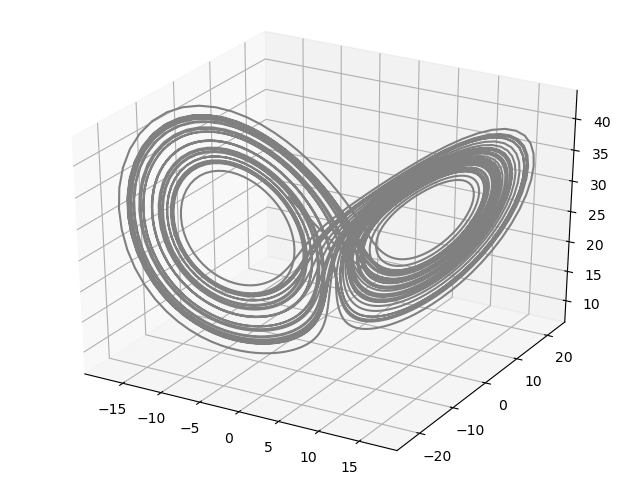
\includegraphics[scale=0.5]{../1.png}
\end{figure}

\begin{figure}[H]
	\centering
	\caption{$x_0 = [6,-7,3]$}
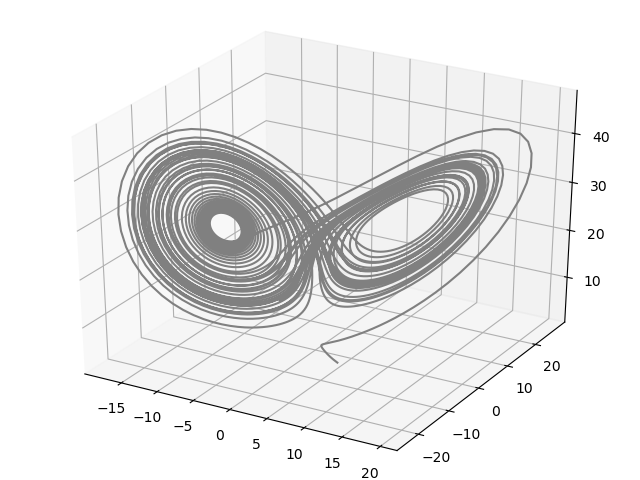
\includegraphics[scale=0.5]{../2.png}
\end{figure}

\begin{figure}[H]
	\centering
	\caption{$x_0 = [0,0,1]$}
	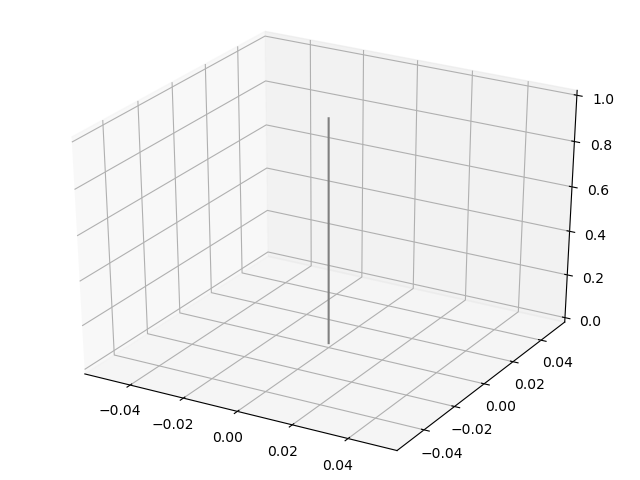
\includegraphics[scale=0.5]{../3.png}
\end{figure}

\begin{figure}[H]
	\centering
	\caption{$x_0 = [8.5,8.5,27]$}
	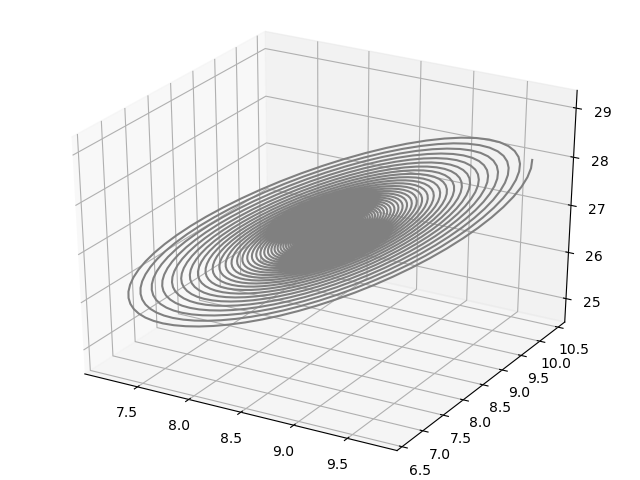
\includegraphics[scale=0.5]{../4.png}
\end{figure}
From these figures we can know there are several types, dependent on the choice of initial value. 1) Converges to a unstable stationary point. 2) Around unstable stationary point 3)Lorentz attractor.


Next we examine the choice of parameters. 

\begin{figure}[H]
	\centering
	\caption{$x_0 = [-10,10,25], \sigma = 28, \rho = 0.5, \beta = 8/3$. When $\rho<1$, we find the system will converge to $[0,0,0]$}
	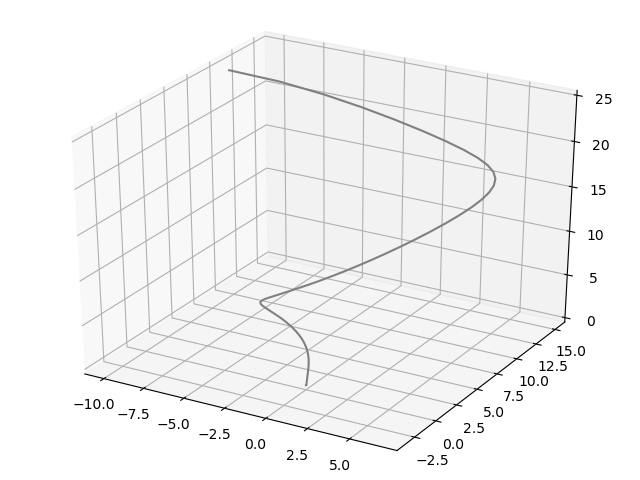
\includegraphics[scale=0.5]{../5.png}
\end{figure}
When $\rho>1$ we find that there are three stationary point $[0,0,0], [\pm\sqrt{\beta(\rho-1)},\sqrt{\beta(\rho-1)},\rho-1]$. Interesting behavior will be found if we choose different $\rho$. 
\begin{figure}[H]
	\centering
	\caption{$x_0 = [-10,10,25], \sigma = 20, \rho = 14, \beta = 8/3$.The system will converge to $[0,0,0]$}
	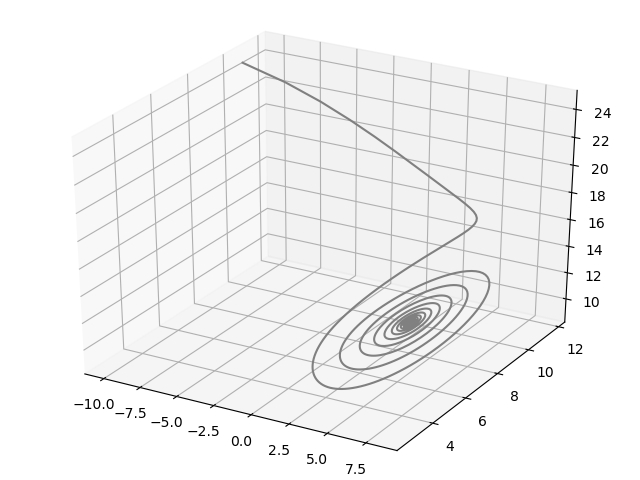
\includegraphics[scale=0.5]{../6.png}
\end{figure}

\begin{figure}[H]
	\centering
	\caption{$x_0 = [-10,10,25], \sigma = 10, \rho = 28, \beta = 100$.The system will converge to $[\pm\sqrt{\beta(\rho-1)},\sqrt{\beta(\rho-1)},\rho-1]$}
	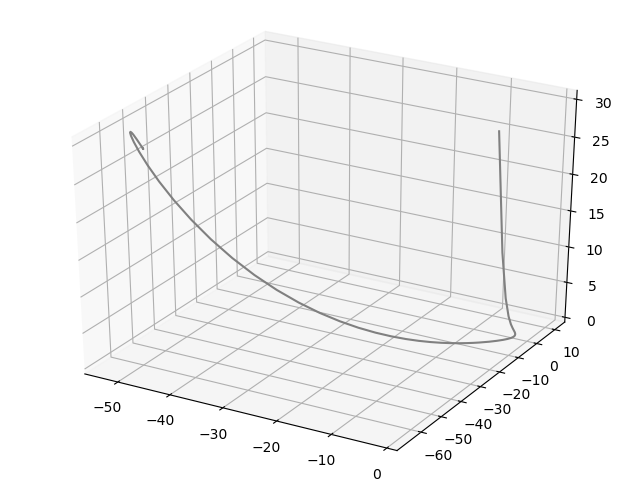
\includegraphics[scale=0.5]{../7.png}
\end{figure}
Extensive experiments show that when $\sigma < \beta +1$, the convergence result is always correct.

When $\sigma>\beta+1$ the result can be either convergent or chaotic.
\end{document}
















Escape special TeX symbols (%, &, _, #, $)